% Copyright (c) 2018 Alexander Bluhm <bluhm@genua.de>
%
% Permission to use, copy, modify, and distribute this software for any
% purpose with or without fee is hereby granted, provided that the above
% copyright notice and this permission notice appear in all copies.
%
% THE SOFTWARE IS PROVIDED "AS IS" AND THE AUTHOR DISCLAIMS ALL WARRANTIES
% WITH REGARD TO THIS SOFTWARE INCLUDING ALL IMPLIED WARRANTIES OF
% MERCHANTABILITY AND FITNESS. IN NO EVENT SHALL THE AUTHOR BE LIABLE FOR
% ANY SPECIAL, DIRECT, INDIRECT, OR CONSEQUENTIAL DAMAGES OR ANY DAMAGES
% WHATSOEVER RESULTING FROM LOSS OF USE, DATA OR PROFITS, WHETHER IN AN
% ACTION OF CONTRACT, NEGLIGENCE OR OTHER TORTIOUS ACTION, ARISING OUT OF
% OR IN CONNECTION WITH THE USE OR PERFORMANCE OF THIS SOFTWARE.

\documentclass[14pt]{beamer}
\usetheme{Frankfurt}
\usepackage{tikz}
\usepackage{graphicx}
\usepackage{tipa}
\author{Alexander Bluhm}
\title{OpenBSD Security Features}
\institute{genua GmbH\\ \url{bluhm@genua.de}\\ \url{bluhm@openbsd.org}}
\date{September 20, 2018}

\begin{document}

\begin{frame}
\titlepage
\end{frame}

\begin{frame}{Agenda}
\setcounter{tocdepth}{1}
\tableofcontents
\end{frame}

\subsection{Avoid malloc(3) Overflow}
\begin{frame}{Avoid malloc(3) Overflow}
\begin{itemize}
    \item {\texttt malloc(nmemb * size)}
    \item {\texttt calloc(nmemb, size)}
    \item {\texttt reallocarray(ptr, nmemb, size)}
    \item Libc does overflow check.
\end{itemize}
\end{frame}

\subsection{Clear Sensitive Memory}
\begin{frame}{Clear Sensitive Memory}
\begin{itemize}
    \item {\texttt bzero(buf, len); free(buf)}
    \item {\texttt explicit\_bzero(buf, len)}
    \item {\texttt freezero(ptr, len)}
    \item {\texttt recallocarray(ptr, oldnmemb, nmemb, size)}
    \item Libc does memset(3).
\end{itemize}
\end{frame}


\section{kbind(2)}

\subsection{Lazy Binding}
\begin{frame}{Lazy Binding}
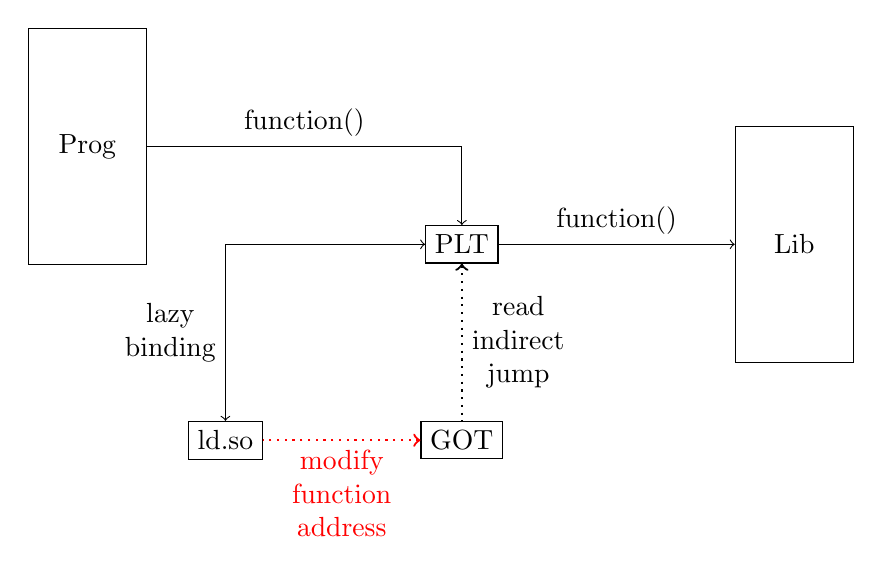
\begin{tikzpicture}
\draw
    node [draw,minimum height=3cm,minimum width=1.5cm] (prog) {Prog};
\draw (prog.east) [->] -- ++(4,0) node [midway,above] {function()} -- ++(0,-1)
    node [draw,below] (plt) {PLT};
\draw (plt.south) [<-,dotted,thick] -- ++(0,-2)
    node [midway,right,align=center] {read\\ indirect\\ jump}
    node [draw,solid,thin,below] (got) {GOT};
in ld.so \draw (got.west) [<-,dotted,thick,red] -- ++(-2,0)
    node [midway,below,align=center] {modify\\ function\\ address}
    node [draw,solid,thin,left,black] (ldso) {ld.so};
\draw (plt.west) [<->] -|
    node [near end,left,align=center] {lazy\\ binding} (ldso);
\draw (plt.east) [->] -- ++(3,0) node [midway,above] {function()}
    node [draw,right,minimum height=3cm,minimum width=1.5cm] (lib) {Lib};
\end{tikzpicture}
\end{frame}

\subsection{Dangerous PLT and GOT}
\begin{frame}{Dangerous PLT and GOT}
\begin{itemize}
    \item Procedure Linkage Table
    \item Global Offset Table
    \item writeable table of code pointers
\end{itemize}
\end{frame}

\subsection{kbind(2) System Call}
\begin{frame}{kbind(2) System Call}
\begin{itemize}
    \item modifies single GOT entry
    \item implicit atomic mprotect(2)
    \item can only called from ld.so(1)
    \item protected by data cookie
\end{itemize}
\end{frame}

\section{pledge(2)}

\subsection{pledge(2) Motivation}
\begin{frame}{pledge(2) Motivation}
\begin{itemize}
    \item restrict system calls
    \item declare functional requirements
    \item tool for programmer
    \item abort process at violation
    \item log problems or attacks
\end{itemize}
\end{frame}

\subsection{Way to pledge(2)}
\begin{frame}{Way to pledge(2)}
\begin{itemize}
    \item studdy existing programs
    \item pattern initialization and main loop
    \item design classes of promises
    \item reimplement some libc functions
    \item pledge nearly all programs
\end{itemize}
\end{frame}

\subsection{pledge(2) Consequences}
\begin{frame}{pledge(2) Consequences}
\begin{itemize}
    \item cleanup program flow
    \item delete (mis-)features
    \item design security model
\end{itemize}
\end{frame}

\subsection{New System Calls}
\begin{frame}{New System Calls}
\begin{itemize}
    \item {\texttt socket(..., SOCK\_DGRAM \textpipe{} SOCK\_DNS, ...) }
    \item {\texttt sendsyslog("log message", 11, LOG\_CONS) }
    \item {\texttt getentropy(buf, buflen) }
\end{itemize}
\end{frame}

\subsection{Use sendsyslog(2)}
\begin{frame}{Use sendsyslog(2)}
\begin{itemize}
    \item {\texttt syslog(3)}, obviously
    \item {\texttt memcpy(3)}
    \item stack protector
    \item ld.so
\end{itemize}
\end{frame}

\section{Priviledge Separation}

\subsection{Priviledge Separation in Processes}
\begin{frame}{Priviledge Separation in Processes}
\begin{itemize}
    \item identify isolated tasks with high risk
    \item {\texttt socketpair(2)}
    \item {\texttt fork(2)}
    \item {\texttt chroot(2)}
    \item {\texttt setuid(2)}
    \item {\texttt pledge(2)}
    \item {\texttt imsg\_init(3)}
    \item file descriptor passing
\end{itemize}
\end{frame}

\subsection{Programs with Privsep}
\begin{frame}{Programs with Privsep}
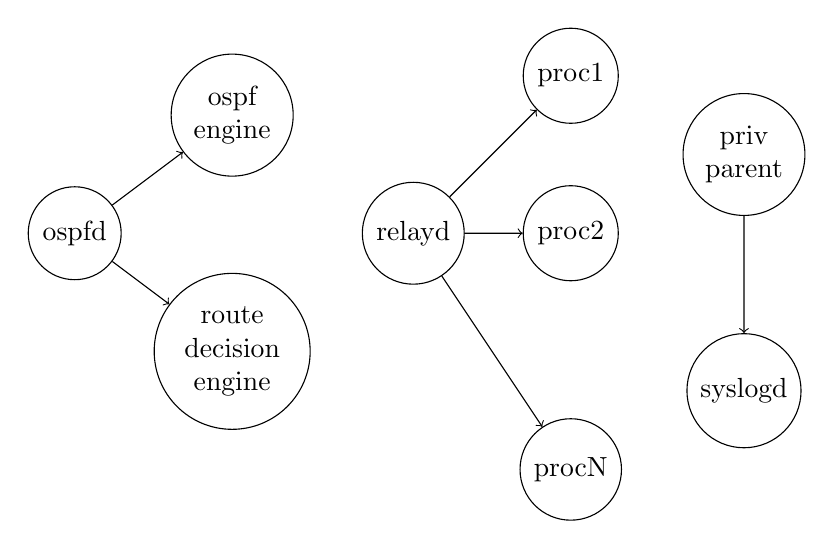
\begin{tikzpicture}
\draw [grow=right,level distance=2cm,sibling distance=3cm]
    (0,0) node [draw,circle,align=center] (ospfd) {ospfd}
    [edge from parent/.style={draw,->}]
    child { node [draw,circle,align=center] (rde) {route\\ decision\\ engine} }
    child { node [draw,circle,align=center] (ospfe) {ospf\\ engine} };
\draw [grow'=right,level distance=2cm,sibling distance=2cm]
    (4.3,0) node [draw,circle,align=center] (relayd) {relayd}
    [edge from parent/.style={draw,->}]
    child { node [draw,circle,align=center] (proc1) {proc1} }
    child { node [draw,circle,align=center] (proc2) {proc2} }
    child { node [draw,circle,align=center,yshift=-1cm] (procn) {procN} };
\draw [grow=down,level distance=3cm]
    (8.5,1) node [draw,circle,align=center] (parent) {priv\\ parent}
    [edge from parent/.style={draw,->}]
    child { node [draw,circle,align=center] (syslogd) {syslogd} };
\end{tikzpicture}
\end{frame}

\subsection{Avoid File Descriptor Exhaustion}
\begin{frame}{Avoid File Descriptor Exhaustion}
\begin{itemize}
    \item getdtablecount()
    \item getdtablesize()
    \item \#define FD\_RESERVE 5
\end{itemize}
\end{frame}

\section{Virtual Address Layout}

\subsection{ASLR Address Space Layout Randomization}
\begin{frame}{ASLR Address Space Layout Randomization}
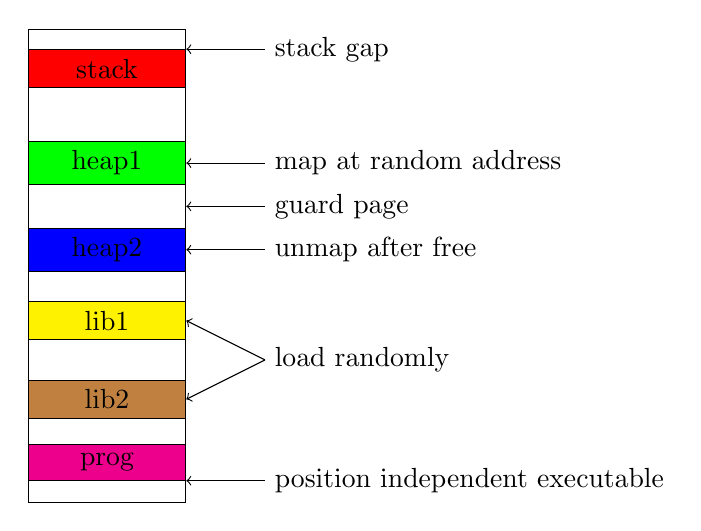
\begin{tikzpicture}
\draw
    (0,0) node [draw,below,minimum width=2cm,minimum height=6cm] (proc) {}
    +(0,-0.5) node [draw,minimum width=2cm,fill=red] (stack) {stack}
    +(0,-1.7) node [draw,minimum width=2cm,fill=green] (heap1) {heap1}
    +(0,-2.8) node [draw,minimum width=2cm,fill=blue] (heap2) {heap2}
    +(0,-3.7) node [draw,minimum width=2cm,fill=yellow] (lib1) {lib1}
    +(0,-4.7) node [draw,minimum width=2cm,fill=brown] (lib2) {lib2}
    +(0,-5.5) node [draw,minimum width=2cm,fill=magenta] (prog) {prog};
\draw (stack.north east) [<-] -- +(1,0) node [anchor=west] {stack gap};
\draw (heap1.east) [<-] -- +(1,0) node [anchor=west] {map at random address};
\path (heap1.east) -- (heap2.east) coordinate [midway] (heap);
\draw (heap) [<-] -- +(1,0) node [anchor=west] {guard page};
\draw (heap2.east) [<-] -- +(1,0) node [anchor=west] {unmap after free};
\path (lib1.east) -- (lib2.east) coordinate [midway] (lib)
    (lib) +(1,0) node [anchor=west] (ldso) {load randomly};
\draw (lib1.east) [<-] -- (ldso.west);
\draw (lib2.east) [<-] -- (ldso.west);
\draw (prog.south east) [<-] -- +(1,0) node [anchor=west]
    {position independent executable};
\end{tikzpicture}
\end{frame}

\subsection{fork+exec}
\begin{frame}{fork+exec}
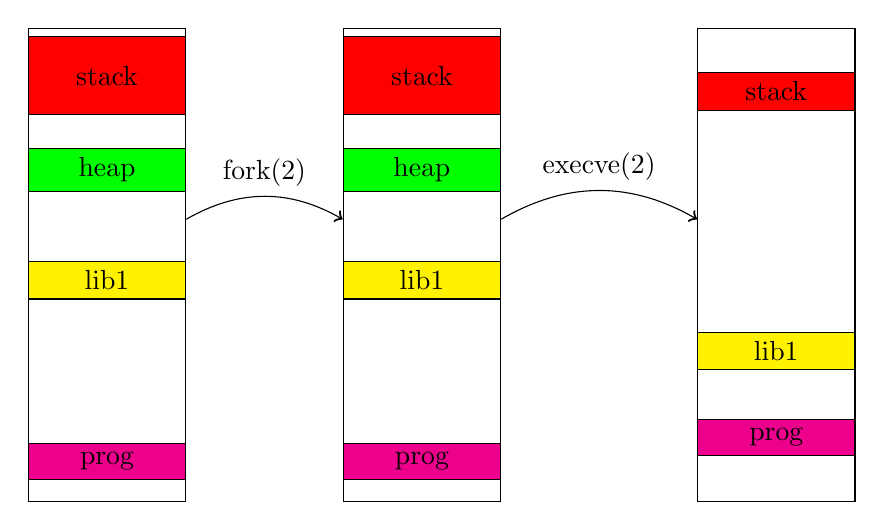
\begin{tikzpicture}
\draw
    (0,0) node [draw,below,minimum width=2cm,minimum height=6cm] (p) {}
    +(0,-0.6) node [draw,minimum width=2cm,fill=red,minimum height=1cm] {stack}
    +(0,-1.8) node [draw,minimum width=2cm,fill=green] {heap}
    +(0,-3.2) node [draw,minimum width=2cm,fill=yellow] {lib1}
    +(0,-5.5) node [draw,minimum width=2cm,fill=magenta] {prog};
\draw
    (4,0) node [draw,below,minimum width=2cm,minimum height=6cm] (f) {}
    +(0,-0.6) node [draw,minimum width=2cm,fill=red,minimum height=1cm] {stack}
    +(0,-1.8) node [draw,minimum width=2cm,fill=green] {heap}
    +(0,-3.2) node [draw,minimum width=2cm,fill=yellow] {lib1}
    +(0,-5.5) node [draw,minimum width=2cm,fill=magenta] {prog};
\draw
    (8.5,0) node [draw,below,minimum width=2cm,minimum height=6cm] (e) {}
    +(0,-0.8) node [draw,minimum width=2cm,fill=red] {stack}
    +(0,-4.1) node [draw,minimum width=2cm,fill=yellow] {lib1}
    +(0,-5.2) node [draw,minimum width=2cm,fill=magenta] {prog};
\draw [->] (p) to [thick,bend left,edge label={fork(2)}] (f);
\draw [->] (f) to [thick,bend left,edge label={execve(2)}] (e);
\end{tikzpicture}
\end{frame}

\subsection{sigreturn(2) from Signal Handler}
\begin{frame}{sigreturn(2) from Signal Handler}
\includegraphics[width=\textwidth]{img/sigreturn.ps}
\end{frame}

\subsection{SROP Signal Return Oriented Programming}
\begin{frame}{SROP Signal Return Oriented Programming}
\includegraphics[width=\textwidth]{img/srop.ps}
\end{frame}

\subsection{Signal Cookie}
\begin{frame}{Signal Cookie}
\includegraphics[width=\textwidth]{img/anti-srop.ps}
\end{frame}

\subsection{Page Protection}
\begin{frame}{Page Protection}
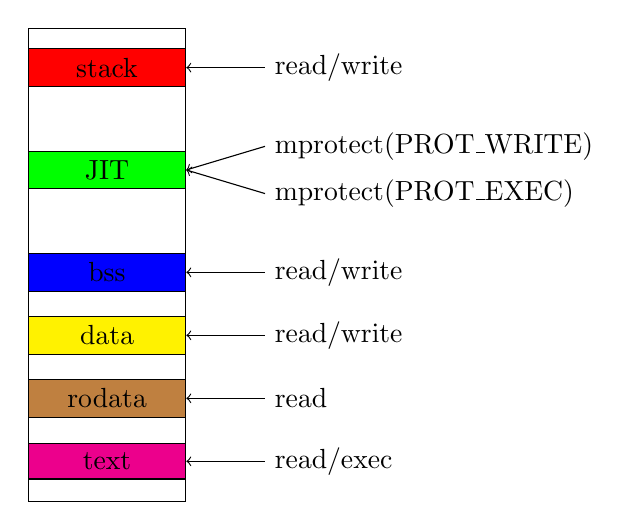
\begin{tikzpicture}
\draw
    (0,0) node [draw,below,minimum width=2cm,minimum height=6cm] (proc) {}
    +(0,-0.5) node [draw,minimum width=2cm,fill=red] (stack) {stack}
    +(0,-1.8) node [draw,minimum width=2cm,fill=green] (jit) {JIT}
    +(0,-3.1) node [draw,minimum width=2cm,fill=blue] (bss) {bss}
    +(0,-3.9) node [draw,minimum width=2cm,fill=yellow] (data) {data}
    +(0,-4.7) node [draw,minimum width=2cm,fill=brown] (rodata) {rodata}
    +(0,-5.5) node [draw,minimum width=2cm,fill=magenta] (text) {text};
\draw (stack.east) [<-] -- +(1,0) node [anchor=west] {read/write};
\draw (jit.east) +(1,0) node [anchor=south west] (mwrite)
    {mprotect(PROT\_WRITE)} (mwrite.west) [->] -- (jit.east);
\draw (jit.east) +(1,0) node [anchor=north west] (mexec)
    {mprotect(PROT\_EXEC)} (mexec.west) [->] -- (jit.east);
\draw (bss.east) [<-] -- +(1,0) node [anchor=west] {read/write};
\draw (data.east) [<-] -- +(1,0) node [anchor=west] {read/write};
\draw (rodata.east) [<-] -- +(1,0) node [anchor=west] {read};
\draw (text.east) [<-] -- +(1,0) node [anchor=west] {read/exec};
\end{tikzpicture}
\end{frame}

\subsection{W\^{}X Write Xor Execute}
\begin{frame}{W\^{}X Write Xor Execute}
\begin{itemize}
    \item ld -z wxneeded
    \item mount -o wxallowed
    \item {\texttt mprotect(PROT\_WRITE \textpipe{} PROT\_EXEC)}
    \item {\texttt mmap(PROT\_WRITE \textpipe{} PROT\_EXEC)}
    \item sysctl kern.wxabort=1
\end{itemize}
\end{frame}

\section{Compiler}

\subsection{Questions}
\begin{frame}{Questions}
\begin{center}
\begin{tikzpicture}
\draw [font=\Huge] node {?};
\end{tikzpicture}
\end{center}
\end{frame}

\subsection{Links}
\begin{frame}{Links}
\begin{itemize}
    \item OpenBSD Innovations
	{\small \url{https://www.openbsd.org/innovations.html}}
    \item deraadt@ Slides about Mitigations
	{\small \url{https://www.openbsd.org/papers/bsdtw.pdf}}
    \item Man Pages at {\small \url{https://man.openbsd.org/}}\\
	\texttt
	pledge(2)
	kbind(2) 
	sendsyslog(2)
	getentropy(2)
	getdtablecount(2)
	
\end{itemize}
\end{frame}

\end{document}
